\chapter{Discussion}


%\section{Evaluation}


%In this paper, we aim to synthesize visually plausible flock motion from video by However, as mentioned in Chapter 1, due to difficulties of obtaining data from real flocks, we do not have ground truth to numerically evaluate our method. As future work, user test can be done by comparing our result with other result generated with naive methods to evaluate our method.


%\section{Bird tracking}


Here, we discuss about limitations and future work of this research. Our system has four limitations:


First, our method uses frame-by-frame optimization as our core method for optimization. An error function is also designed depending on this method. This method makes the optimization can be done in real time for interactive use. However, this approach also makes the generated bird flock having a lack of globally planned trajectory. When optimization is done in every frame, since it only has the information on previous frames, considering data in future frames in advance becomes impossible. This may result in some unnatural results, such as an sudden displacement for avoiding collision. Lacking data in initial frames also makes it difficult to decide positions in those frames. As future work, we can improve the algorithm to optimize globally by reducing computation costs.


Second, bird tracking is also an issue to be solved in this research. Our optimization method can predict three-dimensional position of bird flock in real time. However, the time spend in bird tracking part is the bottleneck of the system. In our experiment, it takes nearly 30 minutes to complete the preprocessing on a 300-frame video by the tracking application we use. Furthermore, manually obtaining track data also takes about 1 minute for 1 bird in a 10-second video. The time needed for manual tracking also limits the number of birds to deal with in a single video. It is fine to track several birds by human eyes. However, when the number of bird increase to like 100 or more, it becomes impossible to track every bird in the flock. Our current system also only allows user to track one bird at a time. As future work, another approach for tracking and synthesizing these dense birds flocks should be proposed. Volume modeling technique in \cite{Fluid} might be useful for modeling dense bird flock.



The third limitation is the method of modeling bird flock. We believe that the method we use to model flocks can be further studied to synthesize better flock motion. In this research, we only consider trajectory smoothness and flock behavior, while environmental effect such as aerodynamics or obstacles is not considered. These factors can be crucial for generating flock motion. In addition, bird locomotion is also not considered while it is a critical part for creating natural flock motion. In addition, although the system allows user to change parameters to modify result, the ability of modification is still quite limited. Although we provide interface for adjusting parameters, the outcome of adjusting these parameters is not instinctive for user. As future work, user interface and parameter tuning can be further improved.


The last limitation in our system is that the assumptions about input video limits the usability of our system. We assume all birds stay in the view field of camera, and the camera stays unmoved during recording. Although it is possible to generate videos that satisfy the assumptions from flock simulation system, it is difficult to have such videos from capturing real bird flock with camera. It is common that birds leave and enter the view field, which is not considered in our system, and bird videos taken with moving camera is also normal. These two assumptions make using real bird video as input difficult, and this is why we make most of the tests with videos generated by flock simulation. More processing needs to be done to eliminate these assumptions.



As future work, we think that the system can be further developed to receive hand-drawn sketch as input. Since human sketch is similar to two-dimension track data obtained from video, as shown in Figure \ref{figure:track}, we think it is possible to develop an similar system that receives hand-drawn sketch and generate results with same method. As we discussed in Chapter 2, motion sketching has become an popular approach to create animations. In our method, we use the track data retrieved from input video. If the track data is replaced by hand-drawn sketch, the time spend in the tracking stage can also be reduced. However, since drawing bird trajectory by hand is not as instinctive as it seems, more works need to be done to achieve the goal. We consider the idea of sketch input as our future work.


\begin{figure}[h]
 \begin{center}
  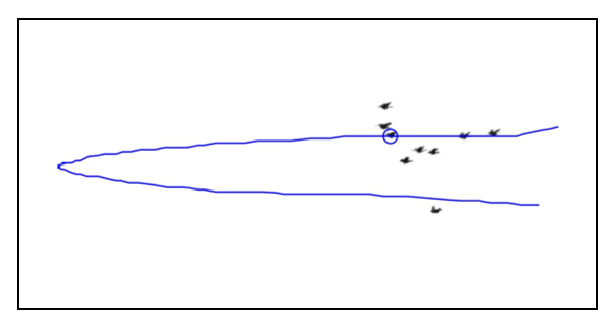
\includegraphics[width=.5\textwidth]{track.eps}
 \end{center}
 \caption{Track trajectory of a bird.}
 \label{figure:track}
\end{figure}